%%%%%%%%%%%%%%%%%%%%%%%%%%%%%%%%%%%%%%%%%
% Contract
% LaTeX Template
% Version 1.0 (December 8 2014)
%
% This template has been downloaded from:
% http://www.LaTeXTemplates.com
%
% Original author:
% Brandon Fryslie
% With extensive modifications by:
% Vel (vel@latextemplates.com)
%
% License:
% CC BY-NC-SA 3.0 (http://creativecommons.org/licenses/by-nc-sa/3.0/)
%
% Note:
% If you are using Apple OS X, go into structure.tex and uncomment the font
% specifications for OS X and comment out the default specifications - this will
% drastically increase how good the document looks. You will now need to
% compile with XeLaTeX.
%
%%%%%%%%%%%%%%%%%%%%%%%%%%%%%%%%%%%%%%%%%

\documentclass[usletter, 12pt]{article}
%%%%%%%%%%%%%%%%%%%%%%%%%%%%%%%%%%%%%%%%%
% Contract Structural Definitions File Version 1.0 (December 8 2014)
%
% Created by: Vel (vel@latextemplates.com)
% 
% This file has been downloaded from: http://www.LaTeXTemplates.com
%
% License: CC BY-NC-SA 3.0 (http://creativecommons.org/licenses/by-nc-sa/3.0/)
%
%%%%%%%%%%%%%%%%%%%%%%%%%%%%%%%%%%%%%%%%%

\usepackage{geometry} % Required to modify the page layout
\usepackage{multicol}
\usepackage{amsmath}
\usepackage{amssymb}

\usepackage[pdftex]{graphicx}
\usepackage{wrapfig}
\usepackage[font=scriptsize, labelfont=bf]{caption}
\usepackage[utf8]{inputenc} % Required for including letters with accents
\usepackage[T1]{fontenc} % Use 8-bit encoding that has 256 glyphs

\usepackage{avant} % Use the Avantgarde font for headings
\usepackage{courier}
\usepackage{xparse}
\usepackage{xcolor}
\usepackage{listings}  % for code verbatim and console outputs

\setlength{\textwidth}{16cm} % Width of the text on the page
\setlength{\textheight}{23cm} % Height of the text on the page
\setlength{\oddsidemargin}{0cm} % Width of the margin - negative to move text left, positive to move it right
\setlength{\topmargin}{-1.25cm} % Reduce the top margin

\setlength{\parindent}{0mm} % Don't indent paragraphs
\setlength{\parskip}{2.5mm} % Whitespace between paragraphs
\renewcommand{\baselinestretch}{1.5}

\definecolor{green}{rgb}{0.18, 0.55, 0.34}

\graphicspath{ {figures/} }
\captionsetup[table]{skip=10pt}

\lstset{language=C, keywordstyle={\bfseries \color{black}}}

% defines algorithm counter for chapter-level
\newcounter{nalg}[section]

%defines appearance of the algorithm counter
\renewcommand{\thenalg}{\thesection .\arabic{nalg}}

% defines a new caption label as Algorithm x.y
\DeclareCaptionLabelFormat{algocaption}{Algorithm \thenalg}

% defines the algorithm listing environment
\lstnewenvironment{pseudocode}[1][] {
    \refstepcounter{nalg}  % increments algorithm number
    \captionsetup{font=normalsize, labelformat=algocaption, labelsep=colon}
    \lstset{
        breaklines=true,
        mathescape=true,
        numbers=left,
        numberstyle=\scriptsize,
        basicstyle=\footnotesize\ttfamily,
        keywordstyle=\color{black}\bfseries,
        keywords={input, output, return, parallel, function, for, to, in, if,
        else, foreach, while, and, or, new, print},
        xleftmargin=.04\textwidth,
        #1
    }
}{}

\renewcommand{\familydefault}{\sfdefault}  % default font for entire document
 % Input the structure.tex file which specifies the document layout and style

%----------------------------------------------------------------------------------------
%   DYNAMIC CONTRACT INFORMATION
%----------------------------------------------------------------------------------------

% Member's information
\newcommand{\project}{Homework - Mastermind}
\newcommand{\Sabbir}{Sabbir Ahmed}

%----------------------------------------------------------------------------------------

\begin{document}

    %----------------------------------------------------------------------------------------
    %   TITLE PAGE
    %----------------------------------------------------------------------------------------

    \begin{titlepage}

        \vspace*{\fill} % Add whitespace above to center the title page content
        \begin{center}

            {\LARGE \project~Report Draft}\\ [1.5cm]

            \today
            
            \vspace*{\fill}

            \Sabbir

        \end{center}
        \vspace*{\fill} % Add whitespace below to center the title page content

    \end{titlepage}

    \section{Description}

        This project emulates a variant of the game "mastermind" on the AVR Dragon. The user will take guesses at the code using the joystick with combinations of up-down-left-right. A wrong input will sound a buzzer (piezoelectric element) and reset the user’s game. Completing the code will light an LED. At this point the game can be reset by pressing the push-button. All inputs will be logged over a serial interface (UART) to a computer reporting the state of the game.

    \section{State Machine Implementation}

        The game is implemented as a state machine, where each successful inputs progresses through the states.

        \begin{figure}[ht]
            \begin{center}
                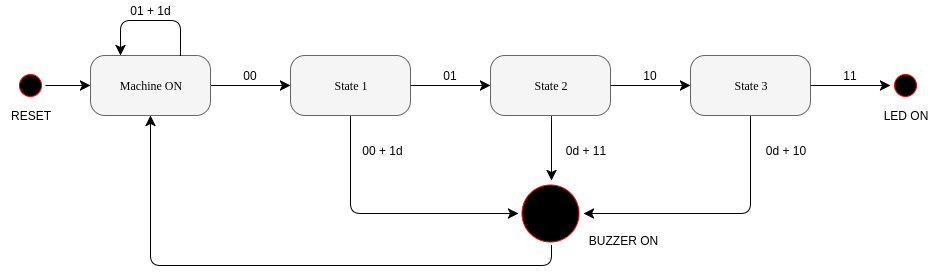
\includegraphics[width=1\textwidth]{figures/state_diagram.png}
                \caption{State Diagram Implementation of the Game with the Secret Code Mapped to 0b00011011} \label{fig:state_diagram}
            \end{center}
        \end{figure}

    \section{Assembly Implementation}

        The program is written in the AVR Assembler in scripts described in Section \ref{sec:code}. 3 registers are used to store the user inputs and compare with the expected inputs. Another register is used to keep track of the number of shifts required for the other registers to be compared accurately.

        The following snippets with visual aids will demonstrate the algorithm used in the program. The following walkthrough sets the secret code as 0b00011011, and the user successfully guesses the sequence.

        \subsection{Initialization}
            As soon as the game is loaded, the directives and labels are loaded with immediate values and the registers are initialized. The ports are initialized as well - PORTB is used for the UP and DOWN joystick inputs, and the LED and buzzer outputs, PORTD is used for the reset push button, and PORTE for the LEFT and RIGHT joystick inputs.

            \begin{table}[h]
                \caption{Values of registers at initialization}
                \centering
                \begin{tabular*}{200pt}{@{\extracolsep{\fill}} c c c}

                \textbf{Register} & \textbf{Before} & \textbf{After} \\
                \hline
                USER & NULL  & NULL \\
                CURSOR & NULL & NULL \\
                REALSTATE & NULL & NULL \\
                NSHIFT & NULL & NULL \\
                \hline
                \textbf{UART} & NULL & NULL \\
                \end{tabular*}
            \end{table}

        \subsection{State Subroutines}
            The program then moves to STATE0, where the secret code is loaded to a register CURSOR, the value 3 is loaded to a register NSHIFT and it waits for the first input. The current state and a delimiter are also transmitted. All the state subroutines consist of identical instructions, with the exception of the immediate values being loaded into the registers and the UART sequences.

\begin{lstlisting}
; STATE0 is the initial state of the game, where the machine waits for the
; user's first input. The correct input progresses the game to the next state,
; and an incorrect input results in the buzzer being triggered.
STATE0:         RCALL TRANSMIT_0            ; transmit '0' for STATE0
                RCALL TRANSMIT_COMMA        ; transmit ','

                LDI CURSOR, SECRET          ; load and mask the secret code
                ANDI CURSOR, 0b11000000     ; into the CURSOR register
                LDI NSHIFT, 3               ; to shift USER BY 3*2 bits
                RCALL RDINPUT               ; get user's input
\end{lstlisting}

            \begin{table}[h]
                \caption{Values of registers before RDINPUT}
                \centering
                \begin{tabular*}{350pt}{@{\extracolsep{\fill}} c c c}

                \textbf{Register} & \textbf{Before} & \textbf{After} \\
                \hline
                USER & NULL  & NULL \\
                CURSOR & NULL & 0b00011011 \& 0b11000000 = 0b00000000 \\
                REALSTATE & NULL & NULL \\
                NSHIFT & NULL & 0b00000010 \\
                \hline
                \textbf{UART} & NULL & 0, \\
                \end{tabular*}
            \end{table}

        \subsection{Reading Inputs}
            RDINPUT waits in a loop for the user's input. Once an input via the joystick is triggered, the program counter moves to the subroutine that has been specified to the input. As per this demonstration, JOYSTICK UP was triggered, leading the program counter to call the JOYSTICKUP subroutine. 

\begin{lstlisting}
; if joystick up was pressed, the UART transmits 'U,' and the current state
; register loads the code for UP which is then shifted
JOYSTICKUP:     RCALL TRANSMIT_U            ; transmit 'U'
                RCALL TRANSMIT_COMMA        ; transmit ','

                LDI USER, UP                ; load joystick input code to USER
                RCALL LSHIFT                ; shift left USER by NSHIFT*2 bits
                RJMP DEBOUNCEUP
                    RET

; waits for user to stop pressing and then returns
DEBOUNCEUP:     SBIC PINB, 6
                    RET
                RJMP DEBOUNCEUP
\end{lstlisting}

            Here, the UART is transmitted with the ASCII value for the initial of the input that was pressed, i.e. `U', followed by the comma delimiter. The USER register is then loaded with the immediate value that was hardcoded as the input, in this case, 0b00000000 for UP.

            \begin{table}[h]
                \caption{Values of registers right after JOYSTICKUP}
                \centering
                \begin{tabular*}{200pt}{@{\extracolsep{\fill}} c c c}

                \textbf{Register} & \textbf{Before} & \textbf{After} \\
                \hline
                USER & NULL  & 0b00000000 \\
                CURSOR & 0b00000000 & 0b00000000  \\
                REALSTATE & NULL & NULL \\
                NSHIFT & 0b00000010 & 0b00000010 \\
                \hline
                \textbf{UART} & 0, & 0,U, \\
                \end{tabular*}
            \end{table}

            The LSHIFT subroutine is then triggered, where the program decrements NSHIFT until it is $\ge$ 1. The USER register is left shifted twice per these iterations. All the joystick input subroutines consist of identical instructions, with the exception of the immediate values being loaded to USER.

\begin{lstlisting}
; left shift the user input to match the position of the states in SECRET
LSHIFT:         LSL USER
                LSL USER                    ; left shift twice per iteration
                DEC NSHIFT                  ; decrement the number of shifts
                CPI NSHIFT, 1
                    BRGE LSHIFT             ; if NSHIFT >= 1, keep looping
                    RET                     ; else, breaks
\end{lstlisting}

            \begin{table}[h]
                \caption{Values of registers after DEBOUNCEUP}
                \centering
                \begin{tabular*}{350pt}{@{\extracolsep{\fill}} c c c}

                \textbf{Register} & \textbf{Before} & \textbf{After} \\
                \hline
                USER & 0b00000000  & 0b00000000 << 3 = 0b00000000 \\
                CURSOR & 0b00000000 & 0b00000000  \\
                REALSTATE & NULL & NULL \\
                NSHIFT & 0b00000010 & 0b00000000 \\
                \hline
                \textbf{UART} & 0,U, & 0,U, \\
                \end{tabular*}
            \end{table}

        \subsection{Evaluating Inputs}
            The program counter then returns to the STATE0 subroutine, and proceeds through the rest of the lines without requiring an input.

\begin{lstlisting}
STATE0:         .
                .
                .
                CLR NSHIFT
                LDI NSHIFT, 3               ; shift REALSTATE to map the codes
                MOV REALSTATE, CURSOR       ; of the joystick inputs
                RCALL RSHIFT
                RCALL EXPINPUT              ; check which input was expected

                RCALL TRANSMIT_COMMA
                RCALL CMPINPUT

                RCALL TRANSMIT_S            ; transmit 'S' for success
                RCALL TRANSMIT_NEWL         ; transmit '\n' to proceed to next
                                            ; state
\end{lstlisting}

            \begin{table}[h]
                \caption{Values of registers right before RSHIFT}
                \centering
                \begin{tabular*}{200pt}{@{\extracolsep{\fill}} c c c}

                \textbf{Register} & \textbf{Before} & \textbf{After} \\
                \hline
                USER & 0b00000000  & 0b00000000 \\
                CURSOR & 0b00000000 & 0b00000000  \\
                REALSTATE & NULL & 0b00000000 \\
                NSHIFT & 0b00000000 & 0b00000010 \\
                \hline
                \textbf{UART} & 0,U, & 0,U, \\
                \end{tabular*}
            \end{table}

            The NSHIFT register is reloaded with the immediate value, this time, to indicate the number of right shifts required for the REALSTATE register. The RCALL subroutine provides an identical procedure as LSHIFT, except for the direction of the bit shifting.

            \begin{table}[h]
                \caption{Values of registers right before EXPINPUT}
                \centering
                \begin{tabular*}{350pt}{@{\extracolsep{\fill}} c c c}

                \textbf{Register} & \textbf{Before} & \textbf{After} \\
                \hline
                USER & 0b00000000  & 0b00000000 \\
                CURSOR & 0b00000000 & 0b00000000  \\
                REALSTATE & 0b00000000 & 0b00000000 >> 3 = 0b00000000 \\
                NSHIFT & 0b00000010 & 0b00000000 \\
                \hline
                \textbf{UART} & 0,U, & 0,U,U,1,S,\textbackslash n \\
                \end{tabular*}
            \end{table}

            The EXPINPUT subroutine is then called, which compares the now shifted REALSTATE to the coded joystick immediate values. Once a match is found, the UART gets transmitted with the ASCII character of the initial of the expected input. The program counter returns to STATE0, and transmits another comma delimiter to the UART.

\begin{lstlisting}
; compares the current state to find the expected output
EXPINPUT:       CPI REALSTATE, UP           ; if current state is 'UP'
                    RCALL TRANSMIT_U        ; transmit 'U'

                CPI REALSTATE, DOWN         ; if current state is 'DOWN'
                    RCALL TRANSMIT_D        ; transmit 'D'

                CPI REALSTATE, LEFT         ; if current state is 'LEFT'
                    RCALL TRANSMIT_L        ; transmit 'L'

                CPI REALSTATE, RIGHT        ; if current state is 'RIGHT'
                    RCALL TRANSMIT_R        ; transmit 'R'

                    RET
\end{lstlisting}

            Finally, the CMPINPUT subroutine is called to compare the USER register with CURSOR. An equal comparison returns the program to the STATE0 subroutine, and proceeds to transmit a successful message to the UART followed by the next state. An unequal comparison branches to BUZZERON and resets the game to STATE0.

\begin{lstlisting}
; compare user's input to the current state and returns if true, else, branches
; to BUZZERON to reset the game
CMPINPUT:       CP CURSOR, USER
                    RET                     ; if equal, return from subroutine
                BREQ BUZZERON               ; else, trigger buzzer
\end{lstlisting}

            The program then proceeds through identical procedure for the remaining states, until the LEDON subroutine is called after the input of a successful sequence.

            \begin{table}[h]
                \caption{Example of values of registers after STATE1}
                \centering
                \begin{tabular*}{200pt}{@{\extracolsep{\fill}} c c c}

                \textbf{Register} & \textbf{Before} & \textbf{After} \\
                \hline
                USER & 0b01000000  & 0b01000000 \\
                CURSOR & 0b01000000 & 0b01000000  \\
                REALSTATE & 0b01000000 & 0b01000000 \\
                NSHIFT & 0b00000001 & 0b00000000 \\
                \hline
                \textbf{UART} & 1,D, & 1,D,D,2,S,\textbackslash n \\
                \end{tabular*}
            \end{table}

    \section{Code} \label{sec:code}

        The assembly code used for the implementation has been attached and provided at the end of the report.

        \subsection{main.asm}
        Contains the state machine implementation of the game and instructions to handle all the inputs and outputs.

        \subsection{uart.asm}
        Contains the specifications for the UART interface.

    \section{Testing and Troubleshooting}

        Because of hardware issues with the AVR Butterfly and its temporary supply issue, the program could not be tested until later in the design timeline. Testing was performed using supplies from peers, with limited availability. Early tests showed failures in the design where the inputs were incorrectly mapped to their ports. After correcting the I/O issues, complex subroutines such as loop shifting were added for elegant solutions and successful tests were performed. The LED was connected to PIN 1 of PORTB and the push button to PIN 7 of PORTD. Additional subroutines were added in the UART instructions later without the available hardware for testing.

    \newpage
    \avrasm{../code/main}{main.asm}

    \newpage
    \avrasm{../code/uart}{uart.asm}


\end{document}
